\documentclass[a4paper,11pt]{report}
\usepackage[T1]{fontenc}
\usepackage[utf8]{inputenc}
\usepackage[polish]{babel}
\usepackage{lmodern}
\usepackage{graphicx}

\title{Roznice w czasie realizacji algorytmów A star, DFS i BFS.}
\author{Arkadiusz Cyktor 200367}

\begin{document}
\maketitle

\begin{figure}
	1. Algorytm A star służy do odnajdywania najwydajniejszej ścieżki w grafie pomiędzy wierzchołkiem A i B. Do jego poprawnej realizacji potrzbna była funkcja heurystyczna, którą zaimplementowałem przez przypisanie wierzchołkom grafu współrzędnych kartezjańskich, co umożliwiło wyliczenie wspomnianej wcześniej funkcji, jako ich wzajemnej odległości w linii prostej. Taki sposób wyznaczania funkcji heurystycznej spełnia warunek, według którego nie powinna ona przeszacowywać odległości pomiędzy wierzchołkami. 
\end{figure}

\begin{figure}
  2. Poniższy wykres przedstawia zależność czasu potrzebnego na znalezienie zadanego wierzchołka grafu od ilości powtórzeń dla algorytmów \textbf{A star} (czerwony), \textbf{DFS} (zielony) i \textbf{BFS} (niebieski). Pomiary były przeprowadzane na grafie zawierającym 30 wierzchołków.
  \\\begin{center} 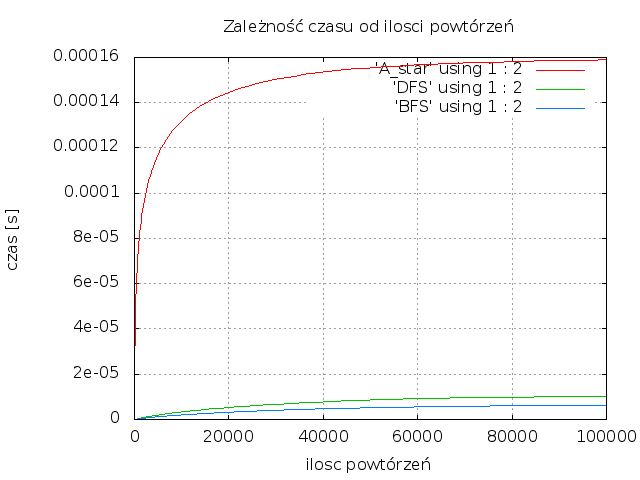
\includegraphics[scale=0.55]{./Razem.png}\end{center}
  Jak widać, wszystkie charakterystyki zmieniają się logarytmicznie, jednak najwięcej czesu na wykonanie obliczeń potrzebuje \textbf{A star}. Różnica pomiędzy przeszukiwaniem \textbf{w szerz}, a \textbf{w głąb} jest niewielka, widać jednak, że ten drugi okazał się wydajniejszy. Takie wyniki są spowodowane zasadniczą różnicą w działaniu wyżej wymienionch algorytmów - w \textbf{BFS} oraz \textbf{DFS} nie bierze się pod uwagę wag krawędzi łączących wierzchołki, co w tak małym grafie skutkuje wyszukaniem w dużo krótszym czasie, jednak wyznaczona ścieżka jest pierwszą znalezioną, a nie najlepszą z możliwych.
\end{figure}

\begin{figure}
  \begin{center}
  Tabela z wynikami pomiarów:\\
  \begin{tabular}{|c|c|c|c|}
  \hline 
  Ilość powtórzeń & Czas - A star & Czas - DFS & Czas - BFS\\
  \hline
  10 & 0 & 0 & 0\\
  \hline
  100 & 0.0001 & 0 & 0\\
  \hline
  1000	&	0.00015 & 0 & 0\\
  \hline
  10000	&	0.000156 & 0.00001 & 0.000006\\
  \hline
  100000 &	0.000159 & 0.0000101 & 0.0000062\\
  \hline
\end{tabular}
\end{center}
\end{figure}
\begin{figure}
  3. Poniższy wykres przedstawia zależność czasu potrzebnego na znalezienie zadanego wierzchołka grafu od ilości wierzchołków w nim zawartych dla algorytmów \textbf{A star} (czerwony), \textbf{BFS} (zielony) i \textbf{DFS} (niebieski).
  \\\begin{center} 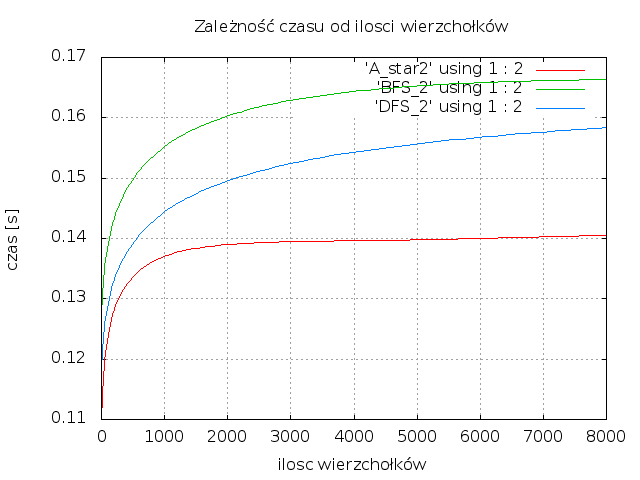
\includegraphics[scale=0.55]{./razem_2.png}\end{center}
  Jak widać, wszystkie charakterystyki zmieniają się logarytmicznie, jednak tym razem porównanie wydjaności algorytmów daje zupełnie inne wyniki - najwięcej czesu na wykonanie obliczeń potrzebuje \textbf{BFS}, po środku znalazł się \textbf{DFS}, a \textbf{A star} okazał się być najwydajniejszym rozwiązaniem. Taka różnica jest spowodowana tym, że dla większych grafów algorytm \textbf{A star} musi wykonać mniej operacji, ponieważ potrafi on odrzucić te krawędzie, które na pewno nie utworzą najwydajniejszej ścieżki - znacznie zawęża to obszar poszukiwań. Natomiast przeszukiwania \textbf{w szerz} i \textbf{w głąb} przeszukują po kolei wszystkie wierzchołki, aż do natrafienia na szukany - jak widać na wykresach takie podejście wymaga dużo większej ilości operacji. 
\end{figure}


\begin{figure}
  \begin{center}
  Tabela z wynikami pomiarów:\\
  \begin{tabular}{|c|c|c|c|}
  \hline 
  Ilość wierzchołków & Czas - A star & Czas - DFS & Czas - BFS\\
  \hline
  10 & 0.112 & 0.12 & 0.129\\
  \hline
  100 & 0.1481 & 0.14563 & 0.15704\\
  \hline
  1000	&	0.13681 & 0.1525 & 0.1643\\
  \hline
  5000	&	0.14000 & 0.1563 & 0.16597\\
  \hline
  8000 &	0.140496 & 0.1584 & 0.166325\\
  \hline
\end{tabular}
\end{center}
\end{figure}
\end{document}